\documentclass{article}
\usepackage[utf8]{inputenc}
\usepackage{float}

\title{Distributed Computing: Documentation}
\author{Zhong-Xi Lu, Angela Mizero, Thomas Van Bogaert}
\date{}

\usepackage{natbib}
\usepackage{graphicx}

\begin{document}

\maketitle

\section{Microservice Oriented Architecture}

\begin{figure}[H]
    \begin{center}
        \makebox[\textwidth]{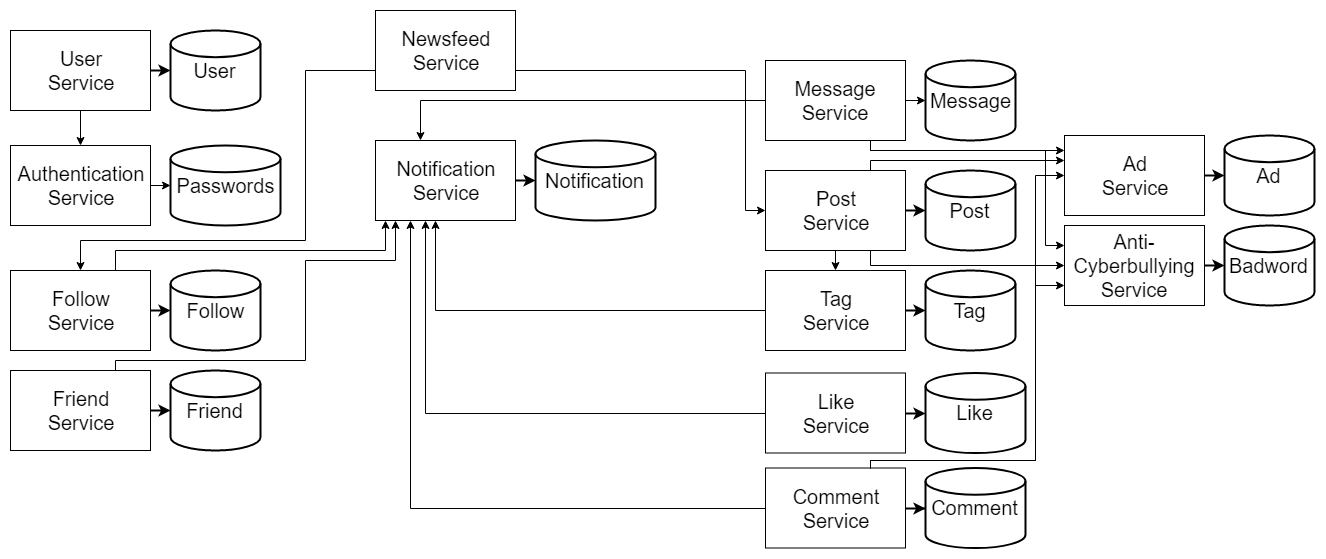
\includegraphics[width=0.8\paperwidth]{images/architecture.png}}
    \end{center}
    \caption{Architecture of core microservices with their interaction}
    \label{fig:arch}
\end{figure}

The core microservices that form the backend of our system can be found in figure \ref{fig:arch}. The interactions, i.e. dependencies, between the different microservices are shown as well. Most of these services also have a corresponding database which is in fact a microservice on its own. More on these services in section \ref{api}.

\begin{figure}[H]
    \begin{center}
        \makebox[\textwidth]{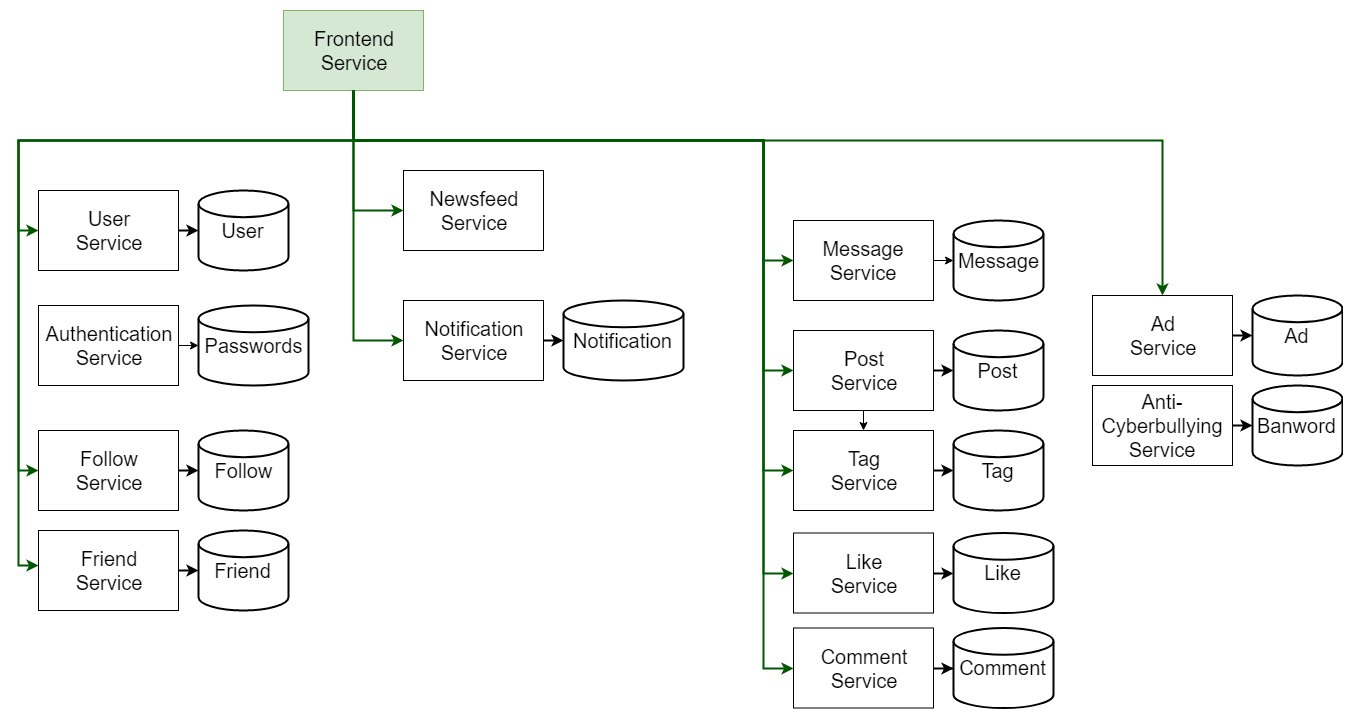
\includegraphics[width=0.8\paperwidth]{images/architecture_frontend.png}}
    \end{center}
    \caption{Architecture of core microservices plus frontend with their interaction}
    \label{fig:arch_frontend}
\end{figure}

On top of all these components, we defined a specific service for the frontend as well (see figure \ref{fig:arch_frontend}). This service will of course communicate with our backend and make use of the provided api. As a side note, each request that is sent from the frontend implicitly goes through the authentication service to verify the user credentials that was stored in a token.

\begin{figure}[H]
    \begin{center}
        \makebox[\textwidth]{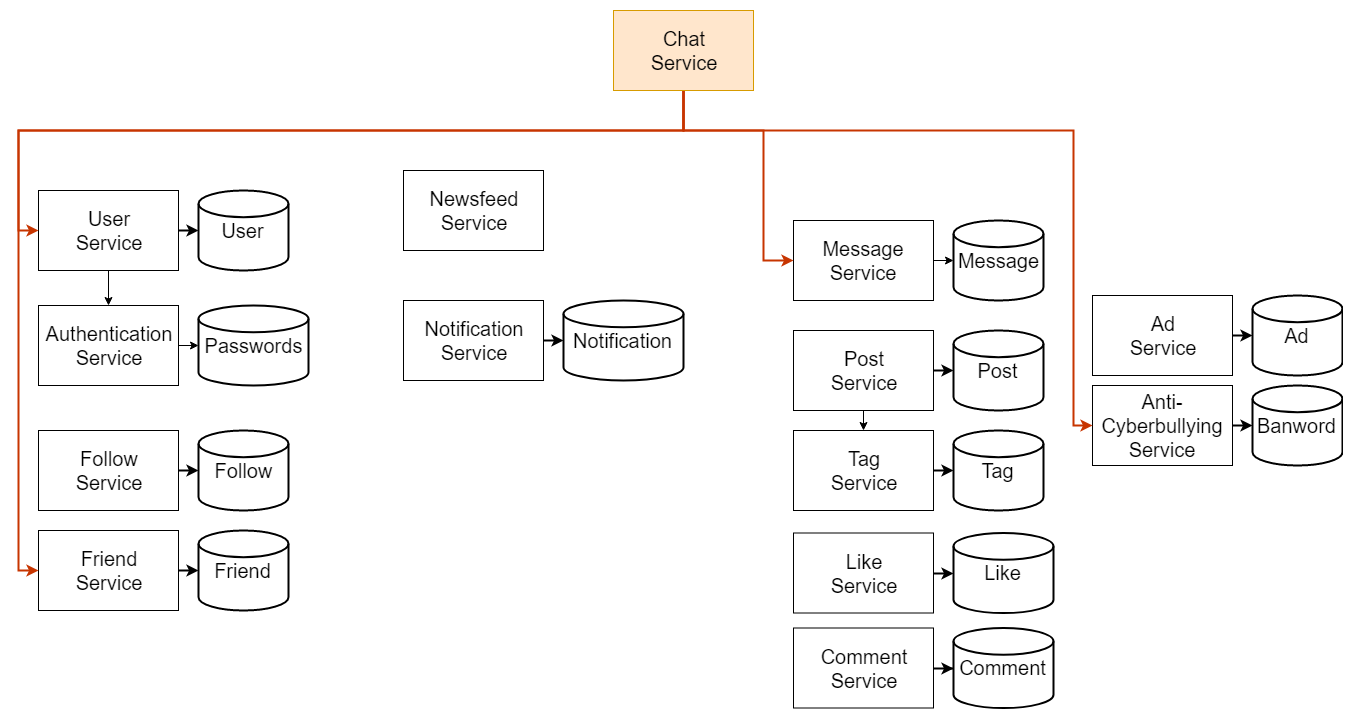
\includegraphics[width=0.8\paperwidth]{images/architecture_chat.png}}
    \end{center}
    \caption{Architecture of core microservices plus chat service with their interaction}
    \label{fig:arch_chat}
\end{figure}

Similarly to the frontend service, there exists a standalone chat application as well. This application is as minimalistic as possible while still providing the basic functionality to login/register and sending messages to your friends.

\begin{figure}[H]
    \begin{center}
        \makebox[\textwidth]{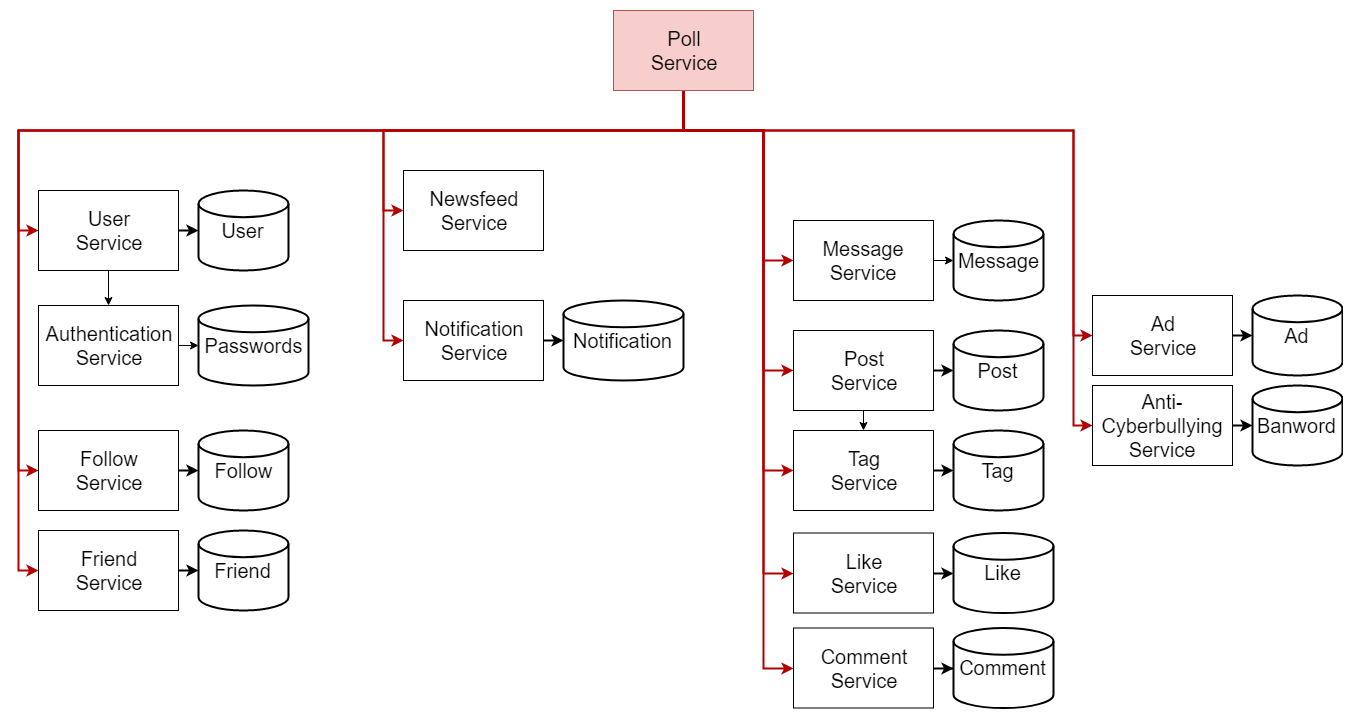
\includegraphics[width=0.8\paperwidth]{images/architecture_poll.png}}
    \end{center}
    \caption{Architecture of core microservices plus poll service with their interaction}
    \label{fig:arch_poll}
\end{figure}

Lastly, we added a separate poll service as well that has the responsibility to poll (send ping request) every service (except user, authentication and notification) and if it detects that a certain service is down for some reason, it will then create a notification for all users respectively.

\section{API Services}
\label{api}

This section will go more into these core microservices by precisely defining their REST API. Note that most of these services also have a ping url.

\begin{description}
    \item [User service:]
    \begin{description}
        \item[]
        \item[In:] POST users (email, username, password)
        \item[Out:] /
        \item[Logic:] Registers or creates a user
        \item[]
    \end{description}
    \begin{description}
        \item[In:] POST users/login (username, password)
        \item[Out:] Response indicating whether the login was successful or not (and return some token if it was successful)
        \item[Logic:] Tries to login a user
        \item[]
    \end{description}
    \begin{description}
        \item[In:] GET users
        \item[Out:] users (user\_id, email, username)
        \item[Logic:] Gets all the users
        \item[]
    \end{description}
    \begin{description}
        \item[In:] GET users/user/username
        \item[Out:] users (user\_id, email, username)
        \item[Logic:] Gets a user by username
        \item[]
    \end{description}
    \begin{description}
        \item[In:] GET users/user\_id
        \item[Out:] user (user\_id, email, username)
        \item[Logic:] Get a particular user
        \item[]
    \end{description}
    \begin{description}
        \item[In:] DELETE users/user\_id
        \item[Out:] /
        \item[Logic:] Deletes a user
        \item[]
    \end{description}
    \begin{description}
        \item[In:] PUT users/user\_id/block
        \item[Out:] /
        \item[Logic:] Blocks a user
        \item[]
    \end{description}
    \begin{description}
        \item[In:] PUT users/user\_id/unblock
        \item[Out:] /
        \item[Logic:] Unblocks a user
    \end{description}
\end{description}

\begin{description}
    \item [Authentication service:]
    \begin{description}
        \item[]
        \item[In:] POST passwords (user\_id, password, is\_admin)
        \item[Out:] /
        \item[Logic:] Adds user and password pair to the database to verify tokens in the future
    \end{description}
    \begin{description}
        \item[]
        \item[In:] PUT passwords (password)
        \item[Out:] /
        \item[Logic:] Updates a user password
    \end{description}
    \begin{description}
        \item[]
        \item[In:] DELETE passwords
        \item[Out:] /
        \item[Logic:] Remove password from the database
    \end{description}
    \begin{description}
        \item[]
        \item[In:] PUT passwords is\_admin
        \item[Out:] Flag indicating whether the user is an admin or not
        \item[Logic:] Check if the user is an admin
    \end{description}
    \begin{description}
        \item[]
        \item[In:] GET verify\_credentials (token)
        \item[Out:] Flag indicating whether the authentication was successful
        \item[Logic:] Tries to authenticate a user by checking their credentials
    \end{description}
\end{description}

\begin{description}
    \item [Message service:]
    \begin{description}
        \item[]
        \item[In:] POST message (contents, sender\_id, receiver\_id)
        \item[Out:] /
        \item[Logic:] Add a new message to DB
        \item[]
        
        \item[In:] GET messages/receiver\_id/sender\_id/$<$amount$>$
        \item[Out:] Messages (content, timestamp, id)
        \item[Logic:] Get messages in conversation between receiver and sender sorted by timestamp
        \item[]
        
        \item[In:] GET messages/user\_id/unread
        \item[Out:] Messages (content, timestamp, id)
        \item[Logic:] Get all unread messages where the user is the receiver
    \end{description}
\end{description}

\begin{description}
    \item [Notification service:]
    \begin{description}
        \item[]
        \item[In:] POST notifications (content, recipients)
        \item[Out:] /
        \item[Logic:] Add notification to DB
        \item[]
    
        \item[In:] GET notifications/notification\_id
        \item[Out:] Notification (ID, timestamp, content)
        \item[Logic:] Get a specific notification
        \item[]
        
        \item[In:] PUT notifications/notification\_id (user\_id)
        \item[Out:] /
        \item[Logic: ] Mark notification as read
        \item[]
        
        \item[In:] GET notifications/user/user\_id 
        \item[Out:] Notifications (ID, timestamp, content)
        \item[Logic:] Get all unread notifications from a specific user
    \end{description}
\end{description}

\begin{description}
    \item [Ad service:]
    \begin{description}
        \item[]
        \item[In:] POST ads (image, categories)
        \item[Out:] /
        \item[Logic:] Add advertisement image to DB (note that the images are actually saved locally instead of in the database; only the image path is stored)
        \item[]
        
        \item[In:] GET ads
        \item[Out:] /
        \item[Logic:] Homepage for the ads service (only accessible for admins)
        \item[]
        
        \item[In:] GET ads/filename
        \item[Out:] Advertisement (image link, category)
        \item[Logic:] Get a specific advertisement based on the filename
        \item[]
        
        \item[In:] POST ads/user/user\_id
        \item[Out:] /
        \item[Logic:] Update (if necessary) the categories of a user (personalized ads)
        \item[]
        
        \item[In:] GET ads/users/user\_id
        \item[Out:] Advertisements (image link, category)
        \item[Logic:] Get ads specifically targeted to a user if any
    \end{description}
\end{description}

\begin{description}
    \item [Anti-Cyberbullying service:]
    \begin{description}
        \item[]
        \item[In:] POST anti\_cyberbullying (words)
        \item[Out:] /
        \item[Logic:] Add new "bad words" to DB
        \item[]
        
        \item[In:] GET anti\_cyberbullying
        \item[Out:] /
        \item[Logic:] Homepage for the anti\_cyberbullying service (only accessible for admins)
        \item[]
        
        \item[In:] GET anti\_cyberbullying/bad\_words
        \item[Out:] All the bad words
        \item[Logic:] Get all the bad words from the database
        \item[]
        
        \item[In:] POST anti\_cyberbullying/contains\_bad\_word (sentence)
        \item[Out:] True if the provided sentence contains one or more bad words, false otherwise
        \item[Logic:] Check if there's a bad word in the sentence
    \end{description}
\end{description}

\begin{description}
    \item [Follow service:]
    \begin{description}
        \item[]
        \item[In:] POST follow (follower\_id, followee\_id)
        \item[Out:] /
        \item[Logic:] User follows another user
        \item[]
    \end{description}
    \begin{description}
        \item[In:] DELETE follow/follower\_id/followee\_id
        \item[Out:] /
        \item[Logic:] Unfollow a user
        \item[]
    \end{description}
    \begin{description}
        \item[In:] GET followees/follower\_id
        \item[Out:] Follows (follower\_id, followee\_id)
        \item[Logic:] Get all users the follower follows
        \item[]
    \end{description}
        \begin{description}
        \item[In:] GET followers/followee\_id
        \item[Out:] Follows (follower\_id, followee\_id)
        \item[Logic:] Get all followers of the user
    \end{description}
\end{description}

\begin{description}
    \item [Friend service:]
    \begin{description}
        \item[]
        \item[In:] POST friend/request (friend\_initiator\_id , friend\_acceptor\_id)
        \item[Out:] /
        \item[Logic:] Create a friend request
        \item[]
    \end{description}
    \begin{description}
        \item[]
        \item[In:] PUT friend/accept (friend\_initiator\_id , friend\_acceptor\_id)
        \item[Out:] /
        \item[Logic:] Accept a friend request
        \item[]
    \end{description}
    \begin{description}
        \item[In:] DELETE friend/friend1\_id/friend2\_id
        \item[Out:] /
        \item[Logic:] Unfriend a user
        \item[]
    \end{description}
    \begin{description}
        \item[In:] GET friend/user\_id/requests
        \item[Out:] Requests (friend\_id)
        \item[Logic:] Get all open friends requests sent to the user
        \item[]
    \end{description}
    \begin{description}
        \item[In:] GET friend/user\_id
        \item[Out:] Friends (friend\_id)
        \item[Logic:] Gets the friends of a user
    \end{description}
\end{description}

\begin{description}
    \item [Newsfeed service:] 
    \begin{description}
        \item[]
        \item[In:] GET newsfeed/user\_id
        \item[Out:] Posts
        \item[Logic:] Get the newsfeed of a user (posts of the people the user is following + own posts)
    \end{description}
\end{description}

\begin{description}
    \item [Post service:]
    \begin{description}
        \item[]
        \item[In:] POST posts (creator, content, tags (usernames))
        \item[Out:] /
        \item[Logic:] Create a new post
        \item[]

        \item[In:] GET posts/user/user\_id
        \item[Out:] Posts (post\_id, creator, timestamp, content)
        \item[Logic:] Get all the posts from a user
        \item[]

        \item[In:] GET posts/post\_id
        \item[Out:] Post (post\_id, creator, timestamp, content)
        \item[Logic:] Get a specific post
        \item[]

        \item[In:] DELETE posts/post\_id
        \item[Out:] /
        \item[Logic:] Delete a specific post
        \item[]
        
        \item[In:] GET posts/stats
        \item[Out:] Number of posts on each day
        \item[Logic:] Get the post statistics, i.e. number of posts on each day
    \end{description}
\end{description}

\begin{description}
    \item [Like service:]
    \begin{description}
        \item[]
        \item[In:] POST likes (post\_id, user\_id)
        \item[Out:] /
        \item[Logic:] User likes a specific post
        \item[]

        \item[In:] GET likes/posts/post\_id
        \item[Out:] Likes (post\_id, user\_id)
        \item[Logic:] Get all the likes of a post
        \item[]
        
        \item[In:] DELETE likes/posts/post\_id (user\_id)
        \item[Out:] /
        \item[Logic:] Undo a like
    \end{description}
\end{description}

\begin{description}
    \item [Tag service:]
    \begin{description}
        \item[]
        \item[In:] POST tags (post\_id, user\_id's)
        \item[Out:] /
        \item[Logic:] Create user tags on a specific post
        \item[]

        \item[In:] GET tags/posts/post\_id
        \item[Out:] Tags (post\_id, user\_id)
        \item[Logic:] Get all the tags on a post
        \item[]
    \end{description}
\end{description}

\begin{description}
    \item [Comment service:]
    \begin{description}
        \item[]
        \item[In:] POST comments (post\_id, creator, content)
        \item[Out:] /
        \item[Logic:] Create a comment on a specific post
        \item[]
        
        \item[In:] GET comments/comment\_id
        \item[Out:] Comment (comment\_id, creator, timestamp, content)
        \item[Logic:] Get a specific comment
        \item[]

        \item[In:] GET comments/posts/post\_id
        \item[Out:] Comments (comment\_id, creator, timestamp, content)
        \item[Logic:] Get all the comments on a post
        \item[]
        
        \item[In:] DELETE comments/comment\_id
        \item[Out:] /
        \item[Logic:] Delete a comment
        \item[]
    \end{description}
\end{description}

\end{document}
